\documentclass[twoside=false,
           twocolumn=false,
           a4paper,DIV=15,
           10pt]{scrartcl}


% using UTF8 as encoding for all files
\usepackage[utf8]{inputenc}

% provides '\includegraphics'
\usepackage{graphicx}

% provides auto-convert eps to pdfs
% \usepackage{epstopdf}

% provides cells spanning multiple rows in tables
\usepackage{multirow}

% American math society, base + symbol package (mathbb and so forth..)
\usepackage{amsmath,amssymb}

% provides double-stroked numbers, for e.g. unit matrix symbol 1
\usepackage{bbm}

% provides support for automated unit typesetting (e.g. 200 GeV)
\usepackage{units}

% provides \toprule etc. for nicer tables
\usepackage{booktabs}

% provides side-figures with text flow around them
\usepackage{wrapfig}

% language support, last option is standard for document
\usepackage[ngerman,english]{babel}

% subimport support for using cascaded \input command (gnuplot epslatex)
\usepackage{import}

%\usepackage[normal]{caption}

% change the (figure,etc.) counter, used for introduction
\usepackage{chngcntr}


% -----------------------------------------------------------
% Set / select font
% -----------------------------------------------------------

% Set the font
\usepackage[T1]{fontenc}

% Latin modern, successor of computer modern with correct umlauts
\usepackage{lmodern}	    



% -----------------------------------------------------------
% Somewhat more complex hyperlink setup 
% -----------------------------------------------------------

% provides extended colors, used here only for links
\usepackage{xcolor}

% link setup as suggested HERE: 
% http://tex.stackexchange.com/questions/823/remove-ugly-borders-around-clickable-cross-references-and-hyperlinks
\usepackage[pdfa,pdfencoding=auto,pdfusetitle
]{hyperref}
\definecolor{dark-red}{rgb}{0.4,0.15,0.15}
\definecolor{dark-blue}{rgb}{0.15,0.15,0.4}
\definecolor{medium-blue}{rgb}{0,0,0.5}
\hypersetup{
    colorlinks, linkcolor={dark-red},
    citecolor={dark-blue}, urlcolor={medium-blue},
    linktocpage=true
}

%
\setcapindent{1.5em}

% -----------------------------------------------------------

\usepackage{listings}

\definecolor{mygreen}{rgb}{0,0.6,0}
\definecolor{mygray}{rgb}{0.5,0.5,0.5}
\definecolor{mymauve}{rgb}{0.58,0,0.82}


\lstset{ %
  basicstyle=
    {\ttfamily\footnotesize},     % the size of the fonts that are used for the code
%  breakatwhitespace=true,          % sets if automatic breaks should only happen at whitespace
%  breaklines=true,                 % sets automatic line breaking
  commentstyle=\color{mygreen},    % comment style
  frame=leftline,
  xleftmargin=0.3em,
  keepspaces=true,                 % keeps spaces in text, useful for keeping indentation of code (possibly needs columns=flexible)
  keywordstyle=\color{blue},       % keyword style
  language=C++,                    % the language of the code
  numbers=none,                    % where to put the line-numbers; possible values are (none, left, right)
  showspaces=false,                % show spaces everywhere adding particular underscores; it overrides 'showstringspaces'
  showstringspaces=true,           % underline spaces within strings only
  showtabs=false,                  % show tabs within strings adding particular underscores
  stringstyle=\color{mymauve},     % string literal style
  tabsize=4,                       % sets default tabsize to 2 spaces
%  title=\lstname,                   % show the filename of files included with \lstinputlisting; also try caption instead of title
  morekeywords=[8]{Spinor,PsiEntry,SU3,Gaugefield,Lattice,LSite,LSiteIter,CommunicationBase}
}

% shorthand to listings inline work
\newcommand\cpp[1]{\lstinline{#1}}

% provides the cref command, automaticly puts "figure, table" etc. in refs
\usepackage{cleveref}


% ============================================================================
% Set a thick line for overfull boxes
% ----------------------------------------------------------------------------

\overfullrule=10pt


% ============================================================================
% list of new commands and shorthands
% ----------------------------------------------------------------------------

% The unit one 
\newcommand{\unitone}{\mathbbm{1}}

% The trace symbol
\DeclareMathOperator{\trace}{Tr}

% The "of order" O
\DeclareMathOperator{\ofOrder}{O}

% point-spread and optical transfer functions
\DeclareMathOperator{\PSF}{PSF}
\DeclareMathOperator{\OTF}{OTF}


% A TODO marker, easily found in the document printout and source code
\newcommand{\TODO}[1]{\textcolor{red}{[TODO]}\textcolor{blue}{(#1)}}
% A comment marker
\newcommand{\cmnt}[1]{\textcolor{orange}{[?: #1]}}

% see http://tex.stackexchange.com/questions/77816/hyperref-not-jumping-to-the-appropriate-location
% sees to that the links point to the top of a figure, not its caption
% do this here so it does not influence the epslatex plots
% done by gnuplot
\usepackage[all]{hypcap}




\usepackage{wrapfig}

\newcommand{\devmarker}{\textit{(development version) }}

% ========================================================================================
% document defintions

\author{\small{Marcel Müller}}
\title{fairSIM quickstart guide} 
\date{\small \today}

% ========================================================================================
% The document itself

\begin{document}

\maketitle

\abstract{This manual provides a short,
step-by-step guide on running a SIM reconstruction by
fairSIM, parameter-setting and trouble-shooting tips,
and a description of our test dataset.
\textbf{Update:} Some features marked \devmarker are only
available when using the current development release of
fairSIM, not the originally published version of our code.
}

\tableofcontents
\newpage



\section{Step-by-step guide}

For datasets of adequate quality, fairSIM offers a
largely automated reconstruction mode, relying as little as
possible on user input. The steps are also labeled in the main
GUI (see \cref{fig-gui}). 

\begin{itemize}
\item \textbf{Open the raw images.} ImageJ / FIJI will
read most microscopy files via BioFormats. Please use
the \emph{split channels} function (either at import
or through FIJI), so that each channel appears as a separate
stack / window.
\item 
\textbf{Start fairSIM}. Choose "new reconstruction"
from the plug-in menu, optionally enabling (verbose) output
of the reconstruction process to the ImageJ log. Alternatively,
an existing set of reconstruction parameters can be loaded.
\item
\begin{minipage}[t]{.55\textwidth}
\textbf{Specify basic parameters}
For a new reconstruction, the first window asks for
basic parameters: 2- or 3-beam 
illumination (2 or 3 bands), the number of 
angles / pattern orientations
used, and the number of phases for each orientation.\\
\emph{By selecting either OMX or Zeiss, these parameters
are set automatically}. 
Also, the ordering of the input image
stack (phases, angles, z-planes) is set accordingly.
\end{minipage}\hfill
\begin{minipage}[t]{.25\textwidth}
\raisebox{-2cm}{
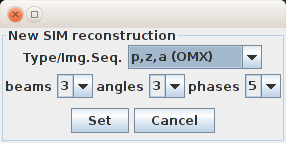
\includegraphics[width=.9\textwidth]{../figures/fairSIM-start}
}
\end{minipage}
\item \textbf{1 - Import the image stack}. In fairSIMs main window,
image selector, choose a raw data stack and click \emph{select}
(clicking the list refreshes available images).
A window opens and allows to:
\begin{itemize}
\item Select the slice to reconstruct, optionally from a wide-field
projection of each slice.
Choose a slice with enough structure well in focus.
\item Set (or override) the physical pixel size.
\item Subtract a constant camera background offset.
\end{itemize}
After a successful import, the image selector shows the currently
imported image name in green. Additionally, a window displays
the raw input data from the selected slice. For 3-beam illumination,
the coarse pattern should clearly be visible on these images.
\item \textbf{1b - Select time-lapse reconstruction} \devmarker
In the "Image selector" field, a second "Timelapse" tab allows for reconstructing
time series of SIM images semi-automatically. The "z-slices" input has
to be set to the number of slices acquired for every time-step, the total
number of time-points is determined automatically. Once a reconstruction
has been completed for one time-step, batch reconstruction and an
automatically updated reconstruction result (recomputed when moving the time slides)
becomes available.
\item \textbf{1c - Image Corrections} \devmarker
The third "Correction" tab allows for a basic (global) correction of varying
intensities between different SIM angles and phases. Variations are estimated
by comparing either averages or medians of the raw images. Large variations
should be cross-checked, as they point to problems in either instrument alignment
or sample properties (check with a known-good sample, e.g. a bead slice, when in doubt).


\item \textbf{2 - Load or approximate the OTF}. An optical transfer function
can either be loaded from file
\footnote{OMX OTF files can be converted to our format with a 
small, additional plugin.}
or approximated. When choosing
\emph{approximate}, the numerical aperture of the objective and the emission wavelength
have to be entered. An additional parameter allows to set a deviation
from the ideal OTF, and is set to a reasonable default.
\item \textbf{3 - Run the parameter estimation}. 
For adequate data sets, the parameter estimation should work
without fine-tuning. Clicking \emph{run}, after some seconds
a window will open and show a visual feedback of the fit process.
Each slice represents one pattern orientation, and should contain
a clearly visible peak found by the fitter (see \cref{fig-fit} for an example and
explanations).
\item Optionally: \textbf{4 - Switch on OTF attenuation for optical sectioning}.\\
OTF attenuation is very helpful when performing single-slice reconstruction
of 3-beam, 3D data.
For the idea, see e.g. \cite{wicker2013-phase1}: The 2D OTF is attenuated
such that frequency components with poor axial resolution (missing cone)
are suppressed and filled from other bands. The attenuation
parameters are described in more detail in the 'Settings' section.
To tweak them, start from the defaults 
and increase/decrease the 'strength' parameter first.

\item \textbf{5 - Run the reconstruction}. After a few seconds,
a new window shows the reconstruction result, and the wide-field
image (with and without Wiener-filtering) for comparison.
Parameters (Wiener filter, apodization cutoff) can be defined in
\emph{setup}.

In the \devmarker Richardson-Lucy (RL) filtering following \cite{perez2016optimal} is available. The type of filtering used and
the iteration count can be accessed via "setup".

The \devmarker version also allows to influence the shape 
of the apotization function $A(k)$ via the "APO bend" parameter $b$. Here
$1.0$ corresponds to a triangular shape, lower numbers push
medium frequency response (roughly as $A(k) = (1-k)^b$ 
with $k=0\dots1$).


\end{itemize}



\begin{figure}
\begin{center}
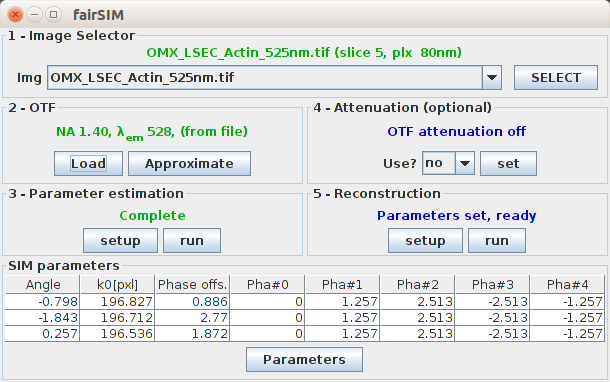
\includegraphics[width=.7\textwidth]{../figures/fairSIM-screenshot}
\end{center}
\caption{Screenshot of fairSIMs main GUI. The numbers label the different
reconstructions steps, incomplete steps show up with red labels. Here,
the first 3 steps have been completed, and the dataset it ready for
reconstruction.}
\label{fig-gui}
\end{figure}




\begin{figure}
\begin{center}
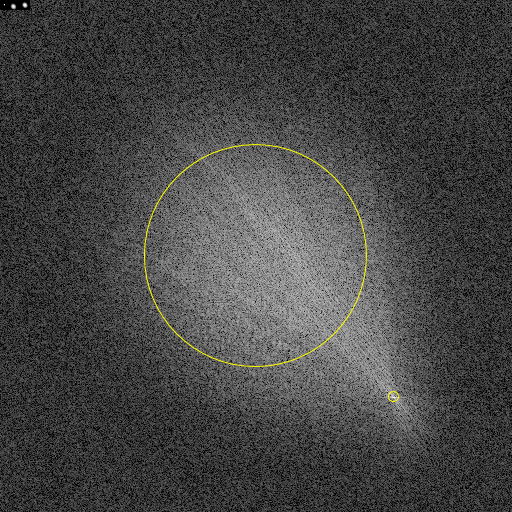
\includegraphics[width=.3\textwidth]{../figures/peakFinder1}
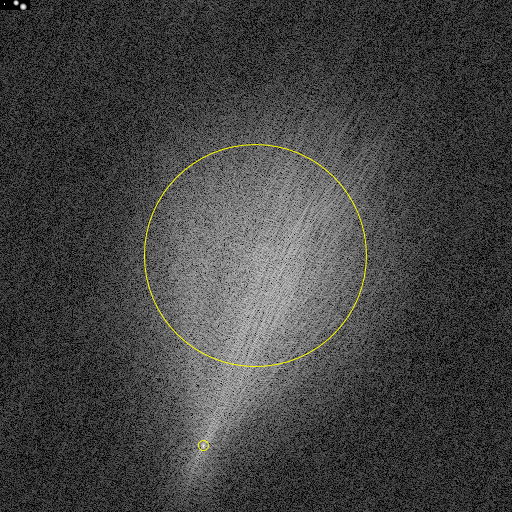
\includegraphics[width=.3\textwidth]{../figures/peakFinder2}
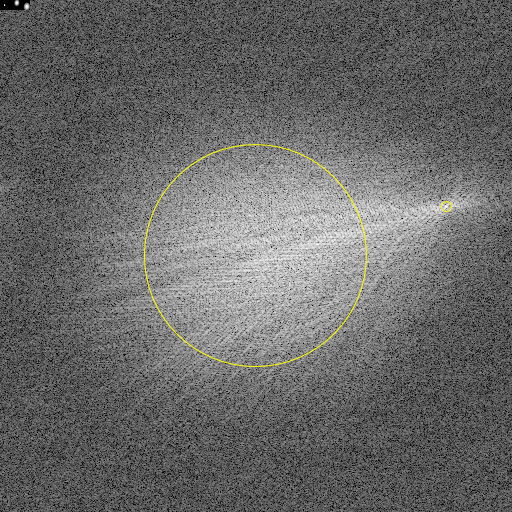
\includegraphics[width=.3\textwidth]{../figures/peakFinder3}
\end{center}

\caption{
Power-spectrum visualization of the cross-correlation used to estimate
reconstruction parameters,
for three pattern orientations. The smaller circles mark where
maxima in the correlation have been found and fitted, the large
center circle marks the low-frequency regions excludes from peak fit
(default at less than 0.6 of the OTF support, settable in the 
parameter estimation menu). The three insets on the top
left visualize the results of the subsequent, iterative, sub-pixel precision
fits. These should show clear elliptic, in most cases circular structure. 
\textbf{If instead the left inset shows noise}, this is a clear indicator
for a failed fit.
}
\label{fig-fit}
\end{figure}

\newpage

\section{Settings and troubleshooting}

Both the parameter estimation and the reconstruction
provide a 'setup' menu to influence the amount of
intermediate result output and to provide 
access to further settings.
FairSIM also supports additional functionality for
advanced users, to assist in cases where more difficult input
datasets are used.

\subsection{Installing and running fairSIM}

After downloading the plugin \verb+.jar+ file, fairSIM is
installed either by copying the file to ImageJs/FIJIs plugin
folder, or by using the \verb+plugin, install+ feature.
Using the menu-based install, some versions of
FIJI display an error message (\verb+WARNING: The PluginClassLoader cannot be reset+).
This is a known bug in FIJI, after a restart of FIJI the plugin
should nonetheless be available. 

When successfully installed, fairSIM can be found 
in the \verb+plugin+ menu, typically towards the end 
of the list (as the name starts with a lowercase letter).


\paragraph{If fairSIM / Fiji hangs:}

In rare cases, fairSIM and/or Fiji hangs, typically after
closing a fairSIM (intermediate) result window. This is
caused by Fiji removing the image window while it is
still in use by fairSIM. To avoid these problems, 
do not close result windows while
fairSIM is active. We are investigating\footnote{If
you are familiar with Java development, and this error
occurs, you can help us by sending in a stack-trace.}
ways to mitigate this problem without 
interfering with the result display.



\subsection{Load / Save}

The SIM reconstruction parameters (displayed by the table
in the main GUI) can be saved to a file, optionally together
with the OTF. The function can be accessed through the
'parameters' menu.

A reconstruction can be loaded from file when starting a
reconstruction from the ImageJ menu.

Please note that currently, shift vectors are not converted
to physical units, i.e. a parameter set for a $512\times 512$
pixel input image will \emph{not} work on a $1024\times1024$
image. If this poses a large drawback, please contact us.

\subsection{Input images}

FairSIM works for reasonable input image sizes. The
most common cases ($512\times512$ and $1024\times1024$ pixels)
are well tested, and are preferred.  Images of arbitrary size 
will be zero-padded to form a square image, 
where the size is a multiple of $32$. The outermost $10$
pixels of all image borders are faded to zero, to avoid
stray components in frequency space.

\subsection{Troubleshooting the parameter estimation}

If the steps described above do not yield a successful parameter estimation,
some advanced settings are available. For users familiar with the
SIM parameter estimation and reconstruction process, they can help
to trouble-shoot the process. 

The parameter estimation is a two-step process working on the
band cross-correlation data: First, the peak in the cross-correlation
is localized, to pixel precision, over the complete image. In a
second step, this localization is iteratively improved to sub-pixel
precision. If it fails, some steps can be taken:

\begin{itemize}
\item The peak localizer outputs the iterative sub-pixel
fit results in the top left corner (see \cref{fig-fit}),
as 3 blocks of $10\times10$ pixels. Especially the first
iteration should show a clear, noise-free point-like structure,
as it covers $\pm 2$ pixels around the initial estimate.
If this is not the case, the initial, coarse localization 
of the peak failed.
\item The initial peak localization assumes the peak
to lie beyond $0.6$ of the maximal OTF support, i.e.
at least a $1.6$-fold resolution improvement. The limit can
be adjusted from the GUI, either up 
(if stray components yield a wrong localization)
or down (if the input data provides less resolution improvement,
see our SLM-SIM test dataset).
\item Increasing the amount of intermediate output provides 
spatial representation
of the overlapping frequency regions used for the cross-correlation
parameter estimation. These should be checked for information 
content (see \cref{fig-otfcommon}).
If there is little structure in the overlapping regions (e.g.
a rather featureless membrane stain), 
the cross-correlation has no information to work on.
\item If this problem occurs for 3-beam data, the parameter
estimation can be switched to work on the first instead of
the second band. This makes the estimation less precise,
but more robust, as the overlap region is much larger.
If the sample shows a clear illumination pattern, but the
parameter estimation fails, try this setting.
\item The parameter estimation, as currently accessible through
the GUI, assumes equi-distant phases. An auto-correlation based
phase estimator for arbitrary phases is 
implemented\cite{wicker2013-phase2}, please contact us if you
need GUI access to this feature.
\end{itemize}


\begin{figure}[b]
\begin{center}
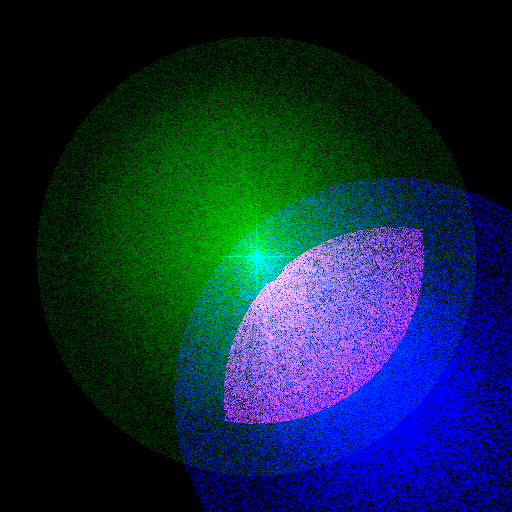
\includegraphics[width=.45\textwidth]{../figures/OtfOverlap_freq}
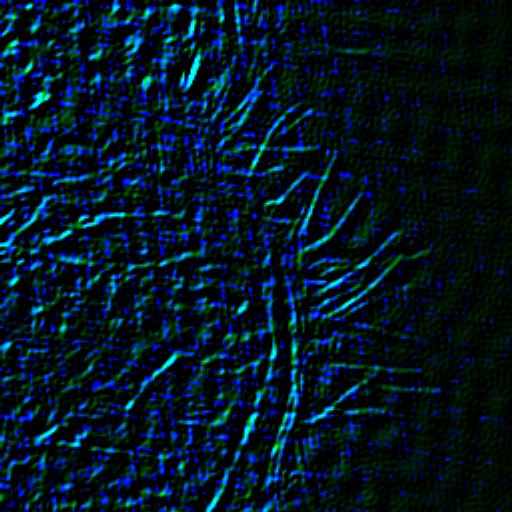
\includegraphics[width=.45\textwidth]{../figures/OtfOverlap_spatial}
\end{center}
\caption{Common region of SIM bands $0$ and $2$ in a 
three-beam reconstruction. Left: Power spectra of
band $\tilde S_0$ (green), shifted band $\tilde S_2$ (blue) and the 
common region (magenta), defined here by 
$h(\vec k),h(\vec k +\vec p)>0.05$, i.e. both bands' OTFs
are above a certain threshold. Right: Composite spatial 
representation of only frequencies from the common region, 
with $S_0$ (green) and $S_2$ (blue), base dataset U2OS actin.
The spatial representation shows that enough information
content is present in both bands to successfully fit
a peak in the correlation.
}
\label{fig-otfcommon}
\end{figure}


\subsection{Settings for the reconstruction}

Wiener filter and apodization are set to reasonable
defaults, but can be tweaked to obtain optimal results.

\begin{itemize}
\item Please note that the Wiener filter
parameter will be squared, i.e. the GUI sets $\omega$, 
not $\omega^2$. 
\item The apodization cut-off is set in
multiples of the OTF cutoff; for datasets where
the resolution improvement deviates from $2\times$,
the parameter can be adjusted.
\item The output can be switched to three modes:
\begin{itemize}
\item Raw output: Includes negative values and performs
no scaling, useful for in-depth analysis
\item Clipped output: Negative values are clipped to zero,
no further scaling is applied
\item Clipped and scaled output (default): Negative values
are clipped to zero, the result is normalized to a 0\dots255
range (but kept at 32bit precision).
\end{itemize}
\item For datasets of thick(er) samples, dialing in the optical
sectioning through the OTF attenuation is often 
the most essential step of acquiring a high-quality reconstruction. 
\begin{itemize}
\item Test different
settings, by varying the \verb+strength+ 
(typically $0.95\dots0.999$) 
and \verb+FWHM+ (typically $0.8\dots2.0)$).
\item The \verb+LSEC1...OMX+ dataset provides
a good example: The attenuation has little effect
on the flat region (lower right side), but a large
effect around the cells core, where there is more
out-of-focus contribution.
\item The Tetraspeck samples are rather flat,
so the attenuation has less effect
\end{itemize}
\end{itemize}

\subsection{Importing or estimating the OTF}

An experimentally determined OTF is preferred. For users of the OMX microscopes, a converter tool is available to extract 2D OTFs from the OTF calibration data provided by the system. For other systems,
a SIM OTF generation tool is in development.

\vspace{1em}

\begin{minipage}[t]{.48\linewidth}
Alternatively, a rough OTF estimate can be provided by fairSIM.
This requires setting the NA and emission wavelength of the 
sample (keep in mind the NA might be reduced due to the
 immersion medium), and allows for setting a "dampening" parameter
$a$ to shift the medium frequency response of the OTF estimation.
The lower $a$ is set, the more medium frequencies are assumed to
be dampened by the optical system. For the example data published
from the OMX system, $a$ has been determined to have a usable 
range of $0.3$ to $0.5$.
\end{minipage}%\hfill
\begin{minipage}[t]{.49\linewidth}
\raisebox{-4cm}{
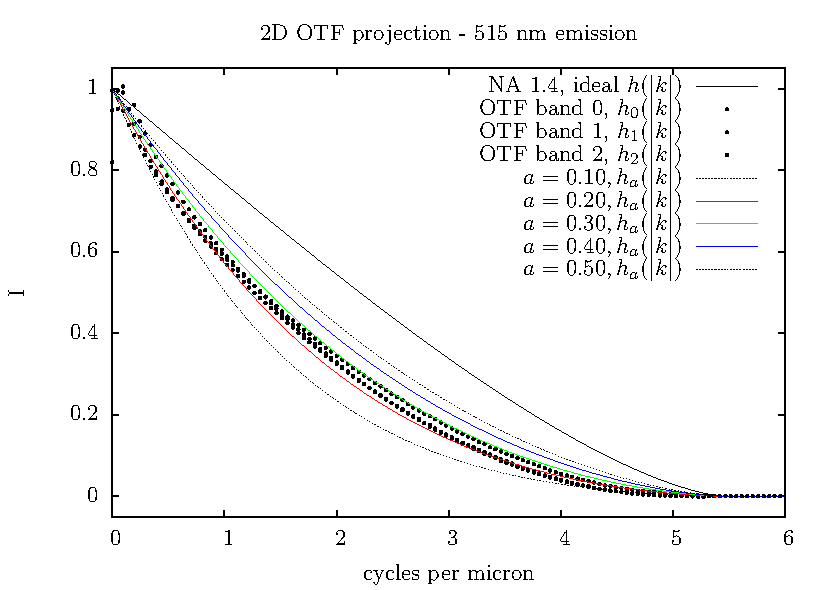
\includegraphics[width=.88\textwidth]{../figures/otf-plot1.pdf}
}
\end{minipage}







\subsection{Setting the amount of intermediate output}

Both the parameter estimation and the reconstruction step can output
a variable amount of intermediate results. 
\paragraph{For the parameter estimation,
these are:}

\begin{itemize}
\item[none] No intermediate results are outputted.
\item[standard] A summary of the fit result
for each pattern orientation is outputted, see \cref{fig-fit}.
This helps to quickly spot failed parameter fits, and is thus
set as the default
\item[most]
Power spectra and spatial domain representation of the overlapping bands used
in the cross-correlation analysis are outputted. For three-beam data, correlations
are outputted for both the lower and the higher band, fit results are shown
for the band selected for the fit.\\
This mode helps to spot if the overlapping, medium frequency regions contain
enough information for a successful fit.
\item[full]
Power spectra of the raw, shifted bands are added to the output. Serious
errors in the band separation should show up in these spectra, but otherwise
the mode should not be needed.
\end{itemize}

\paragraph{For the reconstruction step, these are:}

\begin{itemize}
\item[none] Only the final, reconstructed SR-SIM image is shown
\item[standard] SR-SIM reconstruction, wide-field, wiener-filtered wide-field.
This helps to easily compare the SIM reconstruction and the wide-field image.
\item[more]
Power spectra and spatial domain images of all pattern orientations and bands
are added to the output. This visualizes the information gained through
the SIM process, and also helps to spot errors in single pattern 
directions (uneven illumination, etc.).
\item[most/full]
Currently the same mode, \textit{full} for further additions.
Adds frequency domain representations of the optical transfer functions
to the output. This helps to check if the OTFs fit the data.
\end{itemize}


\section{Modifying, enhancing and automating fairSIM}

Since fairSIM is open-source under GPL, it can freely be used,
but also modified and extended for new purposes. To this end,
the fairSIM source code features a modular design (see \cref{sup-fig-code})
using Java packages:

\begin{itemize}
\item  The \verb+linalg+ package provides 1, 2 and 3-dimensional
vector objects (both real and complex valued) and implements basic
linear algebra routines (additions, scaling). Fourier transformations
are delegated to the \verb+JTransforms+ library, an open source
project featuring a fast, multi-threaded, pure Java 
FFT implementation (similar to FFTW in C/C++).
\item The \verb+sim_algorithm+ package implements the optical transfer
functions, parameter estimations and the actual SIM reconstruction.
\item The \verb+sim_gui+ package provides all components of the graphical 
user interface (see \cref{fig-gui}).
\item The \verb+ImageJ/FIJI+ package allows fairSIM to operate as an
ImageJ plugin. It contains all functions to import images and display
(intermediate and final) results.
\item The \verb+utils+ package provides logging, configuration
file access and routines for easy multi-threading.
\end{itemize}

The modular layout allows one to easily reuse fairSIMs components.
Especially low- and high-level functionality of \verb+sim_algorithm+ can be
used from scripts, without resorting to the GUI. The git repository includes
an example file\footnote{
See \url{https://github.com/fairSIM/fairSIM/blob/v1.0.2/org/fairsim/fiji/TestPlugin.java}
for the complete algorithm and 
\url{https://github.com/fairSIM/fairSIM/blob/v1.0.2/org/fairsim/sim_algorithm/SimAlgorithm.java}
for ready-to-use high level functions.}
, in which a complete reconstruction sequence (setup, coarse and fine
parameter estimation, reconstruction) is run. This file is commented, and
should be easy to adapt to e.g. automated batch data processing.

Also, the data structures and functionality in \verb+linalg+ can
probably be employed to implement new reconstruction methods (e.g. the
current deconvolution-based approaches), as these methods provide more 
convenience than working with pure Java data types.

\paragraph{Documentation}
JAVADOC comments have been used throughout the source code, especially to document
public API functions. Thus, after downloading the source code, the API documentation
can automatically be generated, either by invoking javadoc by hand or through
the provided makefile.



\begin{figure}[ht]
\begin{center}
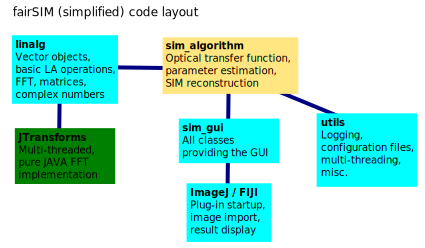
\includegraphics[width=.7\textwidth]{../figures/SketchCodeDiagramm}
\end{center}
\caption{FairSIM modular source code structure}
\label{sup-fig-code}
\end{figure}




%\newpage
\clearpage

\section{Test datasets}

As an additional download, we provide the raw
datasets used to produce the figures in our
publication and the supplemental information.
Here, the parameters used for these reconstructions
are given, so they can serve as an easily accessible
test:

\subsection{OMX examples}

The OMX uses 3-beam illumination, 3 angles, 5 phases,
images are ordered \emph{phases, z, angle}. This is
automatically selected when choosing "OMX". The NA is 1.4,
also set as default. The OTF can either be approximated
or loaded from the provided file. 
The pixel size is $\unit[80]{nm}$,
it should be automatically set from the data file.
The table below provides all further
parameters needed:
\vspace{1em}

\begin{minipage}[l]{.87\textwidth}
\begin{tabular}{lccccc}
File & $\sim \lambda_\text{em.}$ & slice & Background & Att. str. & {\footnotesize FWHM} \\
\hline 
\verb+OMX_LSEC_Actin_525nm.tif+		& \unit[525]{nm} & 5 & 85  & 0.99  & 1.2 \\ 
\verb+OMX_LSEC_Membrane_680nm.tif+	& \unit[680]{nm} & 5 & 350 & 0.995 & 1.2 \\ 
\verb+OMX_Tetraspec200_680nm.tif+	& \unit[680]{nm} & 4 & 80  & 0.98  & 1.2 \\  
\verb+OMX_U2OS_Actin_525nm.tif+\footnote{Good test dataset for optical sectioning}
& \unit[525]{nm} & 7 & --  & 0.9995 & 2.0 \\ 
\verb+OMX_U2OS_Mitotracker_600nm.tif+\footnote{Noisy dataset, set the Wiener filter to
0.09}
& \unit[600]{nm} & 6 & 90  & 0.997  & 1.5 \\ 
\verb+OMX_U2OS_Tubulin_525nm.tif+	& \unit[525]{nm} & 4 & 140 & 0.999 & 1.2 \\ 
\end{tabular}
\end{minipage}


\subsection{Zeiss examples}

The Zeiss Elyra uses 3-beam illumination, 5 angles, 5 phases,
images are ordered \emph{z, angles, phases}. This is automatically
selected when choosing "Zeiss". The NA is 1.4, so the default
value is correct. The pixel size is $\unit[64]{nm}$, and
should be automatically set by from data file. Files are
provided both as $1024\times 1024$ pixels full field-of-view,
and as $512\times 512$ pixels crops for faster analysis / testing.
The table below provides all further parameters

\begin{center}
\begin{tabular}{lccccc}
File & $\sim \lambda_\text{em.}$ & slice & Background &Att. str. & Att. FWHM \\
\hline
\verb+Zeiss_Actin_525nm_*.tif+  & \unit[525]{nm} & 5 & 140 & 0.995 & 1.2 \\
\verb+Zeiss_Mito_600nm_*.tif+   & \unit[600]{nm} & 3 & 140 & 0.995 & 1.2 \\
\end{tabular}
\end{center}

Zeiss example datasets courtesy of Marcus Behringer and Markus Sauer,
University of Würzburg.

\subsection{TIRF-SIM example}

The TIRF SIM dataset was acquired for the work published in \cite{kner2009super},
thus courtesy of Peter Kner.
The illumination parameters are 2-beam, 3 angles, 3 phases, the raw frames 
are in default order. Emission wavelength is approx. \unit[525]{nm}, the
objectives NA is 1.49. The images contain live-cell data captured at 
high frame rates, thus signal levels are somewhat lower (consider setting 
the Wiener filter to e.g. 0.1). It is also important to correct the 
rather high camera offset (background 405), and the region excluded 
from \textbf{parameter fitting has to be set to 0.7}. As a TIRF dataset,
the optical section should of course be turned off.

%\begin{center}
%\begin{tabular}{lccccc}
%File & $\sim \lambda_\text{em.}$ & slice & Background &Att. str. & Att. FWHM \\
%\hline
%\verb+TIRF_Tubulin_525nm.tif+  & \unit[525]{nm} & -- & 405 & -- & -- \\
%\end{tabular}
%\end{center}


\subsection{SLM-SIM example}

Our SLM-SIM example represents a typical dataset from the early stages of our
microscope development. Its quality is not on par with the results
from commercial microscopes. It is included to show that fairSIM can
also handle datasets of simpler, home-build setups.

The SLM-SIM uses 2-beam illumination, with 4 angles and 3 phases, the
images are ordered \emph{phases, angles} (no \emph{z}, as only one slice
is captured). Use the default setting and input the parameters above
accordingly. The NA is $1.2$, the emission wavelength is $\unit[680]{nm}$.
For parameter estimation, the \textbf{fit region has to be adjusted}.
As it defaults to a resolution improvement of $1.6\times$, it should
be lowered to e.g. $0.4$. The images have rather large camera background
offset, so consider setting a background subtraction of $280$ when importing
the stack. Also, the apodization filter can be reduced to $1.6$, as the
full resolution enhancement is not reached.

\bibliographystyle{naturemag}
{\small
\bibliography{./literature}
}
\end{document}
